% -*- root: ../thesis.tex -*-
%!TEX root = ../thesis.tex
% ******************************* Thesis Chapter 7 ****************************

% ----------------------- paths to graphics ------------------------

% change according to folder and file names
\graphicspath{{8/figures/}}
% ----------------------- contents from here ------------------------


\section{Further generalizations and understanding}
The works presented in this thesis only scratched the surface of how helpful mixtures and representations are and opened the way to their identification.
We are still exploring ways to identify larger classes of functions equivalent to scale mixtures.
In particular, the connection with the \acf{MGF} of a distribution is a promising direction since we know how to sample from them \cite{ridout2009generating}.
\ac{MGF} allow us to work not only with continuous but also discrete and multivariate variables.
For example, two of the augmentations of Chapter~\ref{ch:multiclass} do not fit the framework introduced in Chapter~\ref{ch:general} and as shown in Section~\ref{sec:improvemulticlass} are simply \ac{MGF} transformations.
The \ac{MGF} is also an interesting tool to create hierarchical models since scale-mixture are of the form $\sum_{i=0}^\infty e^{tx} p(x)$ or $\int e^{tx}p(x)dx$.
From there, we can plug in P\'olya-Gamma augmentations, using the transformation $t=\log \sigma(x)$, in particular using the property that not only $\sigma(x)$ is augmentable but also $\sigma^n(x)$, for any $n\in \mathbb{R}^+$.
Additional examples of such constructions are shown in this chapter in Sections \ref{sec:heteroscedastic} and \ref{sec:improvemulticlass}.

A potential improvement for augmented models is the identification of marginalizable augmented variables that keep the conditional conjugacy of the model.
For example, in the multi-class model from Chapter~\ref{ch:multiclass}, the augmented variable $\lambda$ can be marginalized, out as shown in Section~\ref{sec:improvemulticlass}.
We can then reduce the dimensionality of the model and avoid tricky situations like the inner loop updates in Chapter~\ref{ch:multiclass}.
This marginalization step can be avoided altogether by identifying from the start the right \ac{MGF}, but the marginalized distributions are sometimes less known.
Augmenting first then marginalizing can then be easier mathematically.

Finally, an unfinished work (despite trying) is to establish convergence rates (error as a function of the number of iterations) for the \ac{CAVI} algorithm and of the correlation of the kernel for the Gibbs sampler.
Experimental results indicate that the error is decreasing as $\|\mathcal{L}^{*} - \mathcal{L}^{t}\|\leq C e^{-t}$, where $t$ is the number of iterations, but we did not manage to form a formal proof.

% TODO add more outlooks

\section{Double bounds for intricate latent GPs}
\label{sec:heteroscedastic}
The model developed in Chapter~\ref{ch:multiclass} paves the ways to work with multi-latent models and hierarchical augmentations.
Another model I worked on but did not publish, is the heteroscedastic regression model,  already explored in \cite{wangGaussianProcessRegression2012,lazaro-gredillaVariationalHeteroscedasticGaussian}.
It consists in simultaneously modeling the mean and variance of a regression likelihood with two latent \ac{GPs} $f$ and $g$.

\subsection{Heteroscedastic Gaussian Likelihood}

A crucial model choice is the function mapping $g$ to the likelihood variance $\epsilon^2$.
The exponential link, i.e. $\epsilon^2(x) = \exp(g(x))$, is the most popular, however to be able to apply our augmentations, we use the link $\epsilon^2(x) = \left(\lambda \sigma(g(x))\right)^{-1}$.
Let's look at the case of the heteroscedastic Gaussian likelihood, defined as:
\begin{align}
    p(y|f,g,\lambda) = \frac{\sqrt{\lambda \sigma(g)}}{\sqrt{2\pi}}\exp\left(-\frac{\lambda \sigma(g)(y-f)^2}{2}\right).\label{eq:hetero_lik}
\end{align}

The augmentations for this likelihood are straightforward and quite similar to the multi-class ones from Chapter~\ref{ch:multiclass}.
\begin{align*}
    \exp\left(-\frac{\lambda\sigma(g)(y-f)^2}{2}\right) =& \exp\left(\frac{\lambda(\sigma(-g) -1)(y-f)^2}{2}\right)\\
    =&\sum_{n=0}^\infty \sigma^n(-g)\Po \left(n~\middle|~\frac{\lambda(y-f)^2}{2}\right),
\end{align*}
where we used the \ac{MGF} of the Poisson distribution.
Now using the P\'olya-Gamma augmentation and the additivity property of P\'olya-Gamma variables, we get the final augmented likelihood:
\begin{align}
    p(y,n,\omega\mid f,g,\lambda) = \frac{\sqrt{\lambda}}{2^n\sqrt{\pi}}\exp\left(\frac{1}{2}\left(g\left(\frac{1}{2}-n\right) - \frac{g^2}{\omega}\right)\right)\PG \left(\omega \mid \half + n, 0\right) \Po \left(n \mid \lambda\frac{(y-f)^2}{2}\right)\label{eq:heteroscedastic}
\end{align}
The interesting part about this augmented likelihood is that although it is conditionally conjugate in $g$, $\omega$ and, $n$, it is unclear how to infer $f$.
It turns out that the Gibbs sampler for this model is very simple.
For the full-conditional of $f$, we marginalize $n$ and $\omega$, return to the original likelihood, which is conditionally conjugate, and perform a \textbf{collapsed step} for the Gibbs sampler with the marginalized full conditional $p(f|g,y)$.

However, as underlined in Section~\ref{sec:cavi}, the \ac{CAVI} updates need the full-conditionals of the model, and the marginalization one of them does not guarantee to get correct updates.
To solve this problem, we need to reverse-engineer how \ac{CAVI} updates are obtained and start with a first bound on the \ac{KL} divergence:
\begin{align*}
    \KL{q(\boldf)q(\boldg)}{p(\boldf,\boldg|\boldy)}\leq& \min_{q(\boldg)}-\expec{q(\boldg)}{\expec{q(\boldf)}{\log p(\boldy|\boldf,\boldg)}} + \KL{q(\boldf)q(\boldg)}{p(\boldf)p(\boldg)}\\
    =& \min_{q(\boldg)}-\expec{q(\boldg)}{\log p(\boldy|\boldg, \bmu^*_f,\bSigma^*_f)} + \KL{q(\boldg)}{p(\boldg)} + \operatorname{KL}_f^* = \mathcal{F}_1.
\end{align*}
$p(\boldy|\boldg, \bmu^*_f, \bSigma^*_f)$ and $\mathrm{KL}^*_f$ are expectations computed with the optimal $q^*(\boldf)=\mathcal{N}\left(\boldf|\bmu_f^*,\bSigma_f^*\right)$.
We can now use the augmentations from equation~\ref{eq:heteroscedastic} on the expected log-likelihood, where we replaced $(y_i-f_i)^2$ by $(y_i - (\bmu_f^*)_i)^2 + (\Sigma_f^*)_{ii}$, and build a second bound.

\begin{align*}
    \mathcal{F}_1 \leq \min_{q(\boldg)q(\bomega,\bn)} \expec{q(\boldg)q(\bomega,\bn)}{\log p(\bomega,\bn,\boldy|\boldg,\bmu_f^*,\bSigma_f^*)} + \KL{q(\boldg)}{p(\boldg)} + \operatorname{KL}_f^*=\mathcal{F}_2
\end{align*}

It is straightforward to find the optimal variational distributions $q^*(\boldg)$ and $q^*(\bomega,\bn)$ minimizing $\mathcal{F}_2$ which allows us to use \ac{CAVI} updates.
Then, injecting the optimal distribution $q^*(\boldg)q(\bomega,\bn)$ in $\mathcal{F}_2$, we can derive the optimal $\bmu_f^*$ and $\bSigma_f^*$, obtainable in closed-form.

This double-bound approach is very similar to \citet{lazaro2011variational}, although they are using the exponential link and need some extra computations.
% TODO add a plot to show it works

\begin{algorithm}[H]
    \caption{\ac{CAVI} Updates for the Heteroscedastic Gaussian likelihood}
    \begin{algorithmic}
        \State \textbf{input:} $q(\boldf,\boldg) = \mathcal{N}(\boldf|\bmu_f,\bSigma_f)\mathcal{N}(\boldg|\bmu_g,\bSigma_g)$, $p(\boldf,\boldg) = \mathcal{N}(\boldf|\bmu^0_f, K)\mathcal{N}(\boldg|\bmu^0_g, K)$, $\boldy$ and $\lambda$.
        \While{convergence criteria is not met}
            \State $\psi^i = \widetilde{\sigma}(q(g^i))$
            \State $\gamma^i = \frac{\lambda}{2} \psi^i  \sqrt{(y^i - \mu_f^i)^2 + \Sigma_f^{ii}}$
            \State $c^i = \sqrt{(\mu_g^i)^2 + \Sigma^{ii}_g}$
            \State $\theta^i = \expec{q(\omega^i|n^i)q(n^i)}{\omega^i} = \frac{0.5 + \gamma^i}{2c^i}\tanh\left(\frac{c^i}{2}\right)$
            \State $\bSigma_f = \left(K^{-1} + \lambda\diag(1-\boldsymbol{\psi})\right)^{-1}$
            \State $\bmu_f = \bSigma_f\left(K^{-1}\bmu_f^0 + \lambda\diag(1 - \boldsymbol{\psi}) \boldy\right)$
            \State $\bSigma_g = \left(K^{-1} + \diag(\btheta)\right)^{-1}$
            \State $\bmu_g = \bSigma_g\left(K^{-1}\bmu_g^0 + \frac{0.5 + \bgamma}{2}\right)$
        \EndWhile
    \end{algorithmic}
    where $q(\boldn, \bomega) = \prod_{i=1}^N \PG(\omega^i|0.5 + n, c^i)\Po(n^i|\gamma^i)$ and $\widetilde{\sigma}(q(g^i)) = \frac{e^{-\mu_g^i/2}}{\sqrt{(\mu_g^i)^2 + \Sigma^{ii}_k} / 2}$ can be seen as a close approximation to $\expec{q(g^i)}{\sigma(-g^i)}$.
    \label{alg:cavi_hetero}
\end{algorithm}

\begin{algorithm}[H]
    \caption{Gibbs sampling for the Heteroscedastic Gaussian likelihood}
    \begin{algorithmic}
        \State \textbf{input:} $\boldf,\boldg$, $p(\boldf,\boldg) = \mathcal{N}(\boldf|\bmu^0_f, K)\mathcal{N}(\boldg|\bmu^0_g, K)$, $\boldy$, $\lambda$.
        \For{$t$ in $1:$ N samples}
            \State Draw $n^i \sim p(n^i|f^i, g^i, \lambda) = \Po(\lambda \sigma(-g^i) \frac{(y^i - f^i)^2}{2})$
            \State Draw $\omega^i \sim p(\omega^i|n^i,g^i) = \PG(0.5 + n^i, |g^i)$
            \State Draw $\boldg \sim p(\boldg|\boldn, \bomega) = \mathcal{N}(\bmu_g,\bSigma_g)$
            \State \quad where $\bSigma_g=  \left(K^{-1} + \diag(\bomega)\right)^{-1}$ and $\bmu_g = \bSigma_g\left(K^{-1}\bmu^0_g + \frac{0.5 - \boldn}{2}\right)$
            \State Draw $\boldf \sim p(\boldf | \boldg, \lambda) = \mathcal{N}(\bmu_f,\bSigma_f)$
            \State \quad where $\bSigma_f = \left(K^{-1} + \lambda\diag(\sigma(\boldg))\right)^{-1}$ and $\bmu_f = \bSigma_f\left(K^{-1}\bmu_f^0 + \lambda\diag(\sigma(\boldg))\frac{\boldy}{2}\right)$
        \EndFor
    \end{algorithmic}
    \label{alg:gibbs_hetero}
\end{algorithm}

A 1-dimensional toy example is shown on Figure~\ref{fig:heteroscedastic} with the results of the inference algorithms.

\begin{figure}
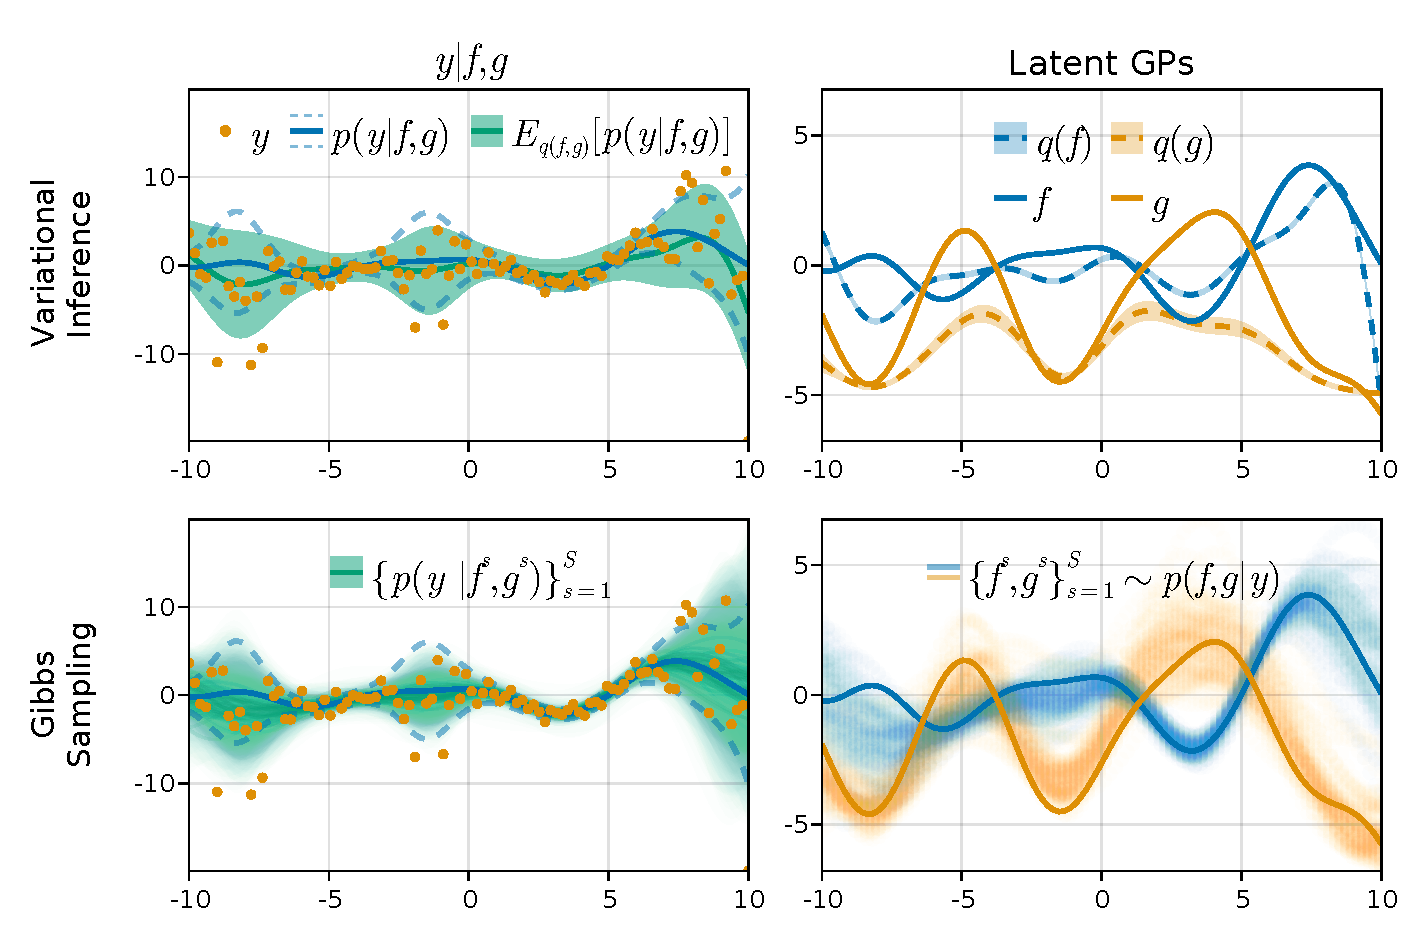
\includegraphics[width=\textwidth]{./chapters/8_discussions/figures/heteroscedastic.pdf}
\caption{Toy example of a heteroscedastic Gaussian regression problem and the resulting inference from Algorithms~\ref{alg:cavi_hetero} and~\ref{alg:gibbs_hetero}.
The left plots show the data in orange and the generating Gaussians (mean with one standard deviation in blue), the green bands show the predictive distributions obtained after posterior inference.
The right plots show the true latent functions $f$ and $g$ used to generate $y$ as well as the inferred posteriors: variational on top (mean with one standard deviation) and samples at the bottom.}
\label{fig:heteroscedastic}
\end{figure}

Note that an implementation as well as detailed derivations can be found in the \href{https://github.com/JuliaGaussianProcesses/AugmentedGPLikelihoods.jl}{AugmentedGPLikelihoods.jl} package \cite{theo_galy_fajou_2022_6347022}.
\subsection{Heteroscedastic Non-Gaussian Likelihood}

We can expand this work to non-Gaussian likelihoods as well.
Let's take the example of the heteroscedastic Laplace likelihood, where we model $\beta(x) = \sqrt{2\beta \sigma(g)}$, where $\beta \in \mathbb{R}^+$.

Similarly to Equation~\ref{eq:hetero_lik} we get the likelihood:
\begin{align*}
    p(y|f,g,\beta) = \frac{\sqrt{\beta\sigma(g)}}{\sqrt{2}}\exp\left(-\sqrt{2\beta(\sigma(g))}|y-f|\right)
    \label{eq:hetero_lik_laplace}
\end{align*}
% TODO Finish these derivations

\section{Using Hamilton Monte Carlo on the augmented model}

The Gibbs sampler in the experiments of Chapters~\ref{ch:classification} and \ref{ch:general} outperforms the state-of-the-art \ac{HMC} algorithm introduced in Section~\ref{sec:hmc}.
A recurrent question I got is:
Is the performance gain due only to the augmentation or to the Gibbs sampler?

First, the augmentation is not in favor of the \ac{HMC} sample due to the increase of dimensionality of the model.
For $N$ observations, we need $KN$ more dimensions (where $K$ depends on the model).
This makes gradients computations and algorithm tuning more expensive.
On the other hand, since the likelihood is simplified to a quadratic problem, the computational complexity of each step can decrease!
The second issue with using \ac{HMC} on the augmented model is that the \ac{pdf} of the prior distribution on augmented variables is not always available in closed-form.
For example, one estimates the probability of a P\'olya-Gamma variable with a truncated alternating series,
Truncated series are not only computationally expensive but can also be biased and unstable!

To have a better idea, Figure~\ref{fig:hmc_vs_gibbs} shows the auto-correlation plots on \ac{GP} regression problem with a Student-t likelihood with 3 degrees of freedom applied on the Boston housing dataset (506 data points, 13 dimensions) \cite{harrison1978hedonic}.
We draw one chain of 2000 samples (plus 500 adaption samples for \ac{HMC} and \ac{NUTS}) for both the original and augmented model.

From the first look, \ac{HMC} applied on the augmented model seems to have a lower auto-correlation.
When using \ac{NUTS}, the gain becomes less clear.
Moreover, the algorithm produces antithetic chains, making it harder to have a proper comparison.
The Gibbs sampler has the smallest intra-chain correlation, but one could argue that negative correlations are more desirable.
However, \ac{HMC} and \ac{NUTS} turned out to be much slower than the Gibbs sampler:
the Gibbs sampler took around 20 sec to run against an average of 12 minutes for \ac{HMC} and \ac{NUTS}.
Perhaps surprisingly, there was no significant time difference between the augmented and original models.

These results should be considered as preliminary, as a simple likelihood was used and the dataset should be considered trivial.

\begin{figure}
    \centering
    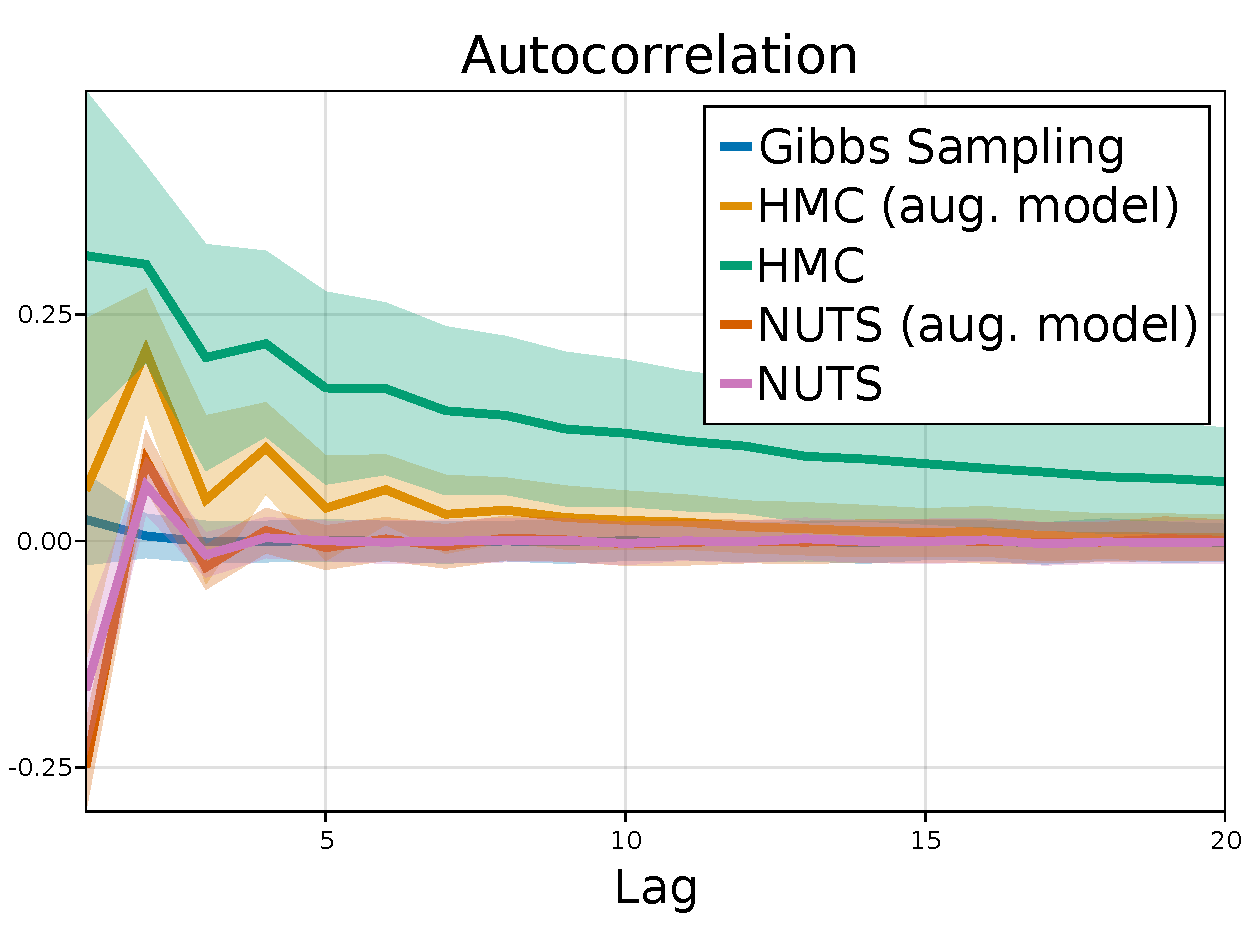
\includegraphics[width=0.5\textwidth]{./chapters/8_discussions/figures/autocorrelation.pdf}
    \caption{Auto-correlation function of the Gibbs sampler, \ac{HMC} and \ac{NUTS} on the augmented model, and \ac{HMC} and \ac{NUTS} on the original model.
    The mean is shown with one standard-deviation over all dimensions.}
    \label{fig:hmc_vs_gibbs}
\end{figure}


\section{Improvements on the Multi-Class Classification}
\label{sec:improvemulticlass}
We recently figured out additional ways to improve the multi-class classification model and the associated inference.
Two of them are listed here

\subsection{Simplex for the multi-class classification}
\label{sec:simplex}
In Chapter \ref{ch:multiclass}, one of the possible concerns regarding the model is that $\lambda$ has the improper prior $p(\lambda) = 1_{[0,\infty)}$, which is a proper measure but is not normalizable.
It should be noted that since the resulting posterior is valid, no problem should arise, but from a purely Bayesian perspective, this can be dissatisfactory.
This improper prior rises from the ill-conditioning of the model.
Given $K$ classes, only $K-1$ latent \ac{GPs} are needed since we have the additional constraint that $\sum_{k=1}^K p(y=k|\boldf) = 1$.
Using this formulation we get the following likelihood:
\begin{align}
    p(y=k|\{f_k\}_{k=1}^{K-1}) = \left\{
        \begin{array}{cc}
            \frac{\sigma(f_k)}{D + \sum_{i=1}^{K-1}\sigma(f_i)}, & \mathrm{if}\; 1 \leq k < K - 1\\
            \frac{D}{D + \sum_{i=1}^{K-1}\sigma(f_i)}, & \mathrm{if}\; k = K - 1 \\
    \end{array}
    \right.,
\end{align}
where $D \in [0, 1]$.
In the coming equations, we set $D=0.5$, which is the equivalent of having the original likelihood with $f_K = 0$.

Using this formulation, the first augmentation that led to an improper prior :
\begin{align*}
    \frac{1}{ \sum_{i=1}^{K} \sigma(f_i)} = \int_0^\infty e^{-\lambda  \sum_{i=1}^{K} \sigma(f_i)}d\lambda
\end{align*}
becomes the known \ac{MGF} of a Gamma distribution with a proper mixture:
\begin{align*}
    \frac{1}{D + \sum_{i=1}^{K-1} \sigma(f_i)} =& \frac{1}{D + \sum_{i=1}^{K-1} \sigma(f_i)} = \frac{1}{D}\frac{1}{1+\frac{1}{D}\sum_{i=1}^{K=1}\sigma(f_i)}\\
    =& \frac{1}{D}\int_0^\infty e^{-\lambda \sum_{i=1}^{K-1} \sigma(f_i)}\Ga \left(1, \frac{1}{D}\right)d\lambda.
\end{align*}
Note that an important condition to use the \ac{MGF} is that $-\sum_{i=1}^{K-1} \sigma(f_i) < D$ which is true as long as $D > 0$.
This condition would not hold with the over-parametrized version which would lead to $D=0$.

From this point, the derivations are identical.
We use the \ac{MGF} of the Poisson distribution and finally the P\'olya-Gamma augmentation.
Unfortunately, we did not run any experiments to explore if one parametrization was more accurate or efficient than another.

Although it is mathematically simpler, a major issue with this model is the choice of $D$.
Since $D$ is fixed, the probability for classes other than $K$ will be bounded $\frac{1}{D + 1}$.
Taking $D=0.5$ would lead to a maximum probability of $2/3$.
On the other hand, if $D=0$, the probability of the class $K$ will always be $0$.
This is not an issue with the softmax link since the exponential function is not bounded.
A potential solution is presented in Section~\ref{sec:scale_multiclass}.

\subsection{Marginalizing out variables}

In the augmentation derived in Chapter~\ref{ch:multiclass}, we add $2K + 1$ new variables per observation: $\lambda$, $\{n_i\}_{i=1}^K$ and $\{\omega_i\}_{i=1}^K$.
However, we can reduce this number to $2K$ and avoid unnecessary inner loops by marginalizing out $\lambda$.
When deriving the augmentations, one ends up with the following augmented likelihood:
\begin{align}
    p(y=k|\{f_i\}_{i=1}^K,\{n_i\}_{i=1}^K,\lambda) = \sigma(f_k) \prod_{i=1}^K \sigma(-f_i)^{n_i} \Po (n_i|\lambda).
\end{align}
We can marginalize out the $\lambda$:
\begin{align}
    \int_{0}^\infty \prod_{i=1}^K \sigma(-f_i)^{n_i} \Po (n_i|\lambda)d\lambda =& \frac{1}{\prod_{i=1}^K n_i!}\int_{0}^\infty \lambda^{\sum_{i=1}^K n_i}e^{-K\lambda}d\lambda \nonumber\\
    =& \frac{K^{-\sum_{i=1}^K n_i}}{\prod_{i=1}^K n_i!}\prod_{i=1}^K \sigma(-f_i)^{n_i} \int_{0}^\infty (K\lambda)^{\sum_{i=1}^K n_i}e^{-K\lambda}d\lambda \nonumber\\
    =& \prod_{i=1}^K\sigma(-f_i)^{n_i}\Gamma(1 + \sum_{i=1}^K n_i) \prod_{i=1}^K \left(\frac{1}{K}\right)^{n_i}\frac{1}{n_i!} \label{eq:NM}
\end{align}

Which is proportional to a negative multinomial $\operatorname{NM}(x_0, \boldsymbol{p})$ with parameters $x_0=1$, $\boldsymbol{p}=\left\{\frac{1}{K}\right\}_{i=1}^K$:
\begin{align*}
    \operatorname{NM}(\bx|x_0,\boldsymbol{p}) = \Gamma\left(\sum_{i=0}^K x_i\right) \frac{p_0^{x_0}}{\Gamma(x_0)}\prod_{i=1}^K \frac{p_i^{x_i}}{x_i!}   
\end{align*}
where $p_0 = 1 - \sum_{i=1}^K p_i$.
Note that $p_0$ is missing in Equation~\ref{eq:NM} and is defined by $p_0= 1 - \sum_{i=1}^K p_i = 1 - \sum_{i=1}^{K}\frac{1}{K} = 0$.
The prior is again non-normalizable, as observed in Section~\ref{sec:simplex}.
Yet, the model is still valid since $p(y,\{f_i\}_{i=1}^K,\{n_i\}_{i=1}^K)$ is normalizable!

More interestingly, all these derivations could have been avoided by noticing that the \ac{MGF} of a negative binomial distribution is given by:
\begin{align*}
    \operatorname{MGF}_{\operatorname{NM}(x_0,\boldsymbol{p})}(\boldsymbol{t}) = \left(\frac{p_0}{1-\sum_{i=1}^K p_k e^{t_i}}\right)^{x_0},
\end{align*}
This makes it even easier to derive the correctly parametrized model proposed in Section~\ref{sec:simplex}.
Quickly identifying the terms in the \ac{MGF}, the augmented likelihood would be:
\begin{align*}
    p\left(y=k,\{n_i\}_{i=1}^{K-1}|\{f_i\}_{i=1}^{K-1}\right) = \frac{\sigma(f_k)}{D}\left(\prod_{i=1}^{K-1}\sigma(-f_i)^{n_i}\right)\operatorname{NM}\left(\boldsymbol{n}\mid 1, \left\{\frac{1}{D+K-1}\right\}_{i=1}^{K-1}\right),
\end{align*}
where we set $\sigma(f_K) = D$.

\subsection{Reformulating the logistic-softmax link}
\label{sec:scale_multiclass}
Another issue from this paper was the logistic-softmax link predictions bounds, in particular with many classes.
Because of the boundedness of the logistic function, the logistic-softmax link needs large values of $f_i$ to reach prediction probabilities close to $1$.
This can be solved by using a scaled logistic function instead.
We add $K$ hyperparameters $\btheta=\{\theta_{i}\}_{i=1}^K$ such that the likelihood becomes
\begin{align*}
    p(y=k|\{f_i\}_{i=1}^K,\btheta) = \frac{\theta_k \sigma(f_k)}{\sum_{i=1}^K \theta_i \sigma(f_i)}.
\end{align*}
The $\btheta$ parameters can be optimized using the \ac{ELBO} with the other hyperparameters.
These can also provide information about each class, a high $\theta_i$ meaning that the $i$-th class has zones of very high confidence.

\begin{algorithm}[H]
    \caption{\ac{CAVI} updates: $\textcolor{sb1}{K}/\textcolor{sb2}{K - 1}$ latent \ac{GPs} for $K$ classes}
    \begin{algorithmic}
    \State \textbf{input:} $q(\boldsymbol{F}) = \prod_{k=1}^{\textcolor{sb1}{K}/\textcolor{sb2}{K - 1}} q(\boldf_k|\bmu_k, \bSigma_k)$, $p(\boldsymbol{F} = \prod_{k=1}^{\textcolor{sb1}{K}/\textcolor{sb2}{K - 1}} p(\boldf_k|\bmu_0, K)$, $Y=\{\boldy^i\}_{i=1}^N$ (one-hot encoded)
    \While{convergence criteria is not met}
        \State $c^i_k = \sqrt{(\mu^i_k)^2 + \Sigma_k^{ii}}$
        \State $p^i_k = \textcolor{sb1}{\frac{\widetilde{\sigma}(q(f_k^i))}{K}}/\textcolor{sb2}{\frac{\widetilde{\sigma}(q(f_k^i))}{D + K - 1}}$
        \State $\bgamma^i = \expec{q(\boldsymbol{n}^i)}{\boldsymbol{n}^i} = \frac{\boldsymbol{p}^i}{1 - \sum_{i=1}^K p^i_k}$
        \State $\theta_k^i = \expec{q(\omega_k^i)}{\omega_k^i} = \frac{y_k^i + \gamma_k^i}{2c_k^i}\tanh\left(\frac{c_k^i}{2}\right)$
        \State $\bSigma_k = \left(K^{-1} + \diag(\boldsymbol{\theta}_k)\right)^{-1}$
        \State $\bmu_k = \bSigma_k\left(K^{-1}\bmu_0 + \frac{\boldy_k - \bgamma_k}{2}\right)$
    \EndWhile
    \end{algorithmic}
    where $q(\boldsymbol{N}, \bOmega) = \prod_{i=1}^N \PG(\bomega^i|\boldy^i + \boldsymbol{n}^i, \boldsymbol{c}^i)\mathrm{NM}(\boldsymbol{n}^i|1, \boldsymbol{p}^i)$ and $\widetilde{\sigma}(q(f_k^i)) = \frac{e^{-\mu_k^i/2}}{\sqrt{(\mu_k^i)^2 + \Sigma^{ii}_k} / 2}$ is an approximation to the $\sigma(-f^i_k)$.
    \label{alg:cavi_multiclass}
\end{algorithm}

The Gibbs sampling updates are of course very similar:
\begin{algorithm}[H]
    \caption{Gibbs sampling updates: $\textcolor{sb1}{K}/\textcolor{sb2}{K - 1}$ latent \ac{GPs} for $K$ classes}
    \begin{algorithmic}
    \State \textbf{input:} $\boldsymbol{F} = \{\boldf_k\}_{k=1}^K$, $p(\boldsymbol{F}) = \prod_{k=1}^{\textcolor{sb1}{K}/\textcolor{sb2}{K - 1}} p(\boldf_k|\bmu_0, K_{XX})$, $Y=\{\boldy^i\}_{i=1}^N$ (one-hot encoded)
    \For{$t$ in 1: \# samples}
        \State Draw $\boldsymbol{n}^i \sim p(\boldsymbol{n}^i|\boldsymbol{F}) = \mathrm{NM}(1, \boldsymbol{p}^i)$ where 
        $p_k^i = \textcolor{sb1}{\frac{\sigma(-f_k^i)}{K}}/\textcolor{sb2}{\frac{\sigma(-f_k^i)}{D + K - 1}}$
        \State Draw $\omega_k^i \sim p(\omega_k^i|f_k^i, n_k^i, y_k^i) = \PG(y_k^i + n^i_k, |f_k^i|)$
        \State Draw $\boldf_k \sim p(\boldf_k|\bomega_k,\boldsymbol{n}_k, \boldsymbol{Y}) = \mathcal{N}(\boldm_k, \boldsymbol{S}_k)$
        \State where $\boldsymbol{S}_k = \left(K^{-1} + \diag(\bomega_k)\right)^{-1}$ and $\boldm_k = \boldsymbol{S}_k\left(K^{-1}\bmu_0 + \frac{\boldy_k - \boldsymbol{n}_k}{2}\right)$
    \EndFor
    \end{algorithmic}
    \label{alg:gibbs_multiclass}
\end{algorithm}

% TODO Give proper introduction to the algorithms explicit models under this setup

Note that an implementation as well as detailed derivations can be found in the \href{https://github.com/JuliaGaussianProcesses/AugmentedGPLikelihoods.jl}{AugmentedGPLikelihoods.jl} package \cite{theo_galy_fajou_2022_6347022}.

\section{Sampling from a sparse augmented model}

Another work in progress regards the sampling of sparse \ac{GPs} models.
Being able to sample directly from the augmented model is ideal as it allows recovering samples from the original posterior $p(\boldf|\bX,\boldy)$.
Unfortunately, this does not transfer when using sparse \ac{GPs}.
Naively using an additional set of points, without using the \citet{Titsias2009} assumption, leads to an algorithm with complexity $\mathcal{O}((N+M)^3)$, defeating the point of the algorithm.
However, one can resort to mixing a variational approach to sampling.
Instead of optimizing the parameters of the distribution $q(\boldu)$, we consider a free-form variational distribution defined as a collection of samples $\{\boldu_i\}_{i=1}^T$ coming from the optimal variational distribution $q^*(\boldu)$ \cite{hensmanMCMCVariationallySparse2015}.
In other words, we want to sample from the optimal $q^*(\boldu)$ which minimizes the \ac{KL} divergence with $p(\boldu|\bX,\boldy)$:
\begin{align*}
    \log q^*(\boldu) = \expec{p(\boldf|\boldu)}{\log p(\boldy|\boldf)} + \log p(\boldu) + C.
\end{align*}
The straightforward option is to use \ac{HMC} as in \cite{hensmanMCMCVariationallySparse2015} to sample from this objective.
We can also derive a Gibbs sampling algorithm to draw samples from this objective using our previous work on augmentations.

In our new setting the optimal distribution is defined as $q(\boldf,\boldu,\bOmega) = p(\boldf|\boldu)q(\boldu, \bOmega)$, where $\bOmega$ denotes the set of augmented variables.
Note that, unlike in the traditional \ac{VI} setting, $\boldu$ and $\bOmega$ are not assumed to be independent.
From there, $\bOmega$, $\boldu$ and $\boldf$ are sampled one after another using the optimal distributions $q^*(\bOmega|\boldu,\boldf)$ and $q^*(\boldu,\boldf|\bOmega)$.
Note that we sample $\boldu$ and $\boldf$ together since they are highly correlated.
To identify the optimal conditional distributions, we look at the minimizer of the conditional \ac{KL} divergence, e.g. $q^*(\bOmega|\boldu,\boldf) = \arg_{q} \min \KL{q(\bOmega|\boldu,\boldf)}{p(\bOmega|\boldu,\boldf,\boldy,\bX)}$.
The obvious minimizer here is to set $q^*=p$, and thanks to the augmentations, we know $p(\bOmega|\ldots)$ in closed-form.
We can perform a similar approach for $q^*(\boldu,\boldf|\bOmega)$.
The only parameters left are the hyperparameters (omitted in the previous equations), which can be sampled by using the more traditional \ac{HMC} algorithm in a separate Gibbs sampling step.
The advantage of this approach is that no gradients are necessary as all full-conditionals are known in closed-form and we do not need any expectation over the log-likelihood.
This opens up more possibilities over more complex problems like the multi-class or heteroscedastic one where computing expectations would be a limitation.
For medium-sized datasets this can even prove to outperform the \ac{CAVI} algorithm as it has the same convergence speed but does not suffer from the mean-field assumption on the variational parameters.
Hopefully, this work should be released in the near future.

\section{Limits}

As pointed out in chapters about augmentations, working with augmented models has its own issues.
The main one being of course having to identify potential augmentations in a given model and to compute lengthy derivations to arrive at the right result.
The idea generalization of using \ac{MGF} is promising, but is also limited.
Often terms need to be rearranged, identities need to be used to reach something usable.
This is feasible for someone with expertise, but it is a complicated problem to automatize the process, in the context of probabilistic programming for example.
Current progress in symbolic programming could eventually help in this direction.
By having a lookup table of augmentable functions and the ability to transform equations, this process can be automatized.

Another issue is the variational distribution $q(\boldf, \bOmega)$ (or $q(\boldu, \bOmega)$) optimized on the augmented model is not as accurate as the variational distribution $q(\boldf)$ (or $q(\boldu)$) optimized on the original model.
Interestingly the difference of bound comes exclusively from the mean-field assumption between $q(\boldf)$ and $q(\bOmega)$.
We can even identify these bound differences via the interpretation of \citet{} as missing terms from a Taylor series.

Since the predictive results prove to be almost as good and that the difference of bounds is not always significant, this gives us a strong sign that the two set of variables are naturally strongly decorrelated and this would give a strong clue on why the Gibbs sampling and \ac{CAVI} updates tend to be so efficient.
In fact, the work of \citet{gorinovaAutomaticReparameterisationProbabilistic2020} mentioned in the introduction aims at finding a perfect balance between two parametrizations by ensuring that the posterior is as close as possible to a multivariate Gaussian with independent dimensions.




% ---------------------------------------------------------------------------
% ----------------------- end of thesis sub-document ------------------------
% ---------------------------------------------------------------------------
